\documentclass[10pt,a4paper]{article}
\usepackage[utf8]{inputenc}
\usepackage{amsmath}
\usepackage{amsfonts}
\usepackage{amssymb}
\usepackage{makeidx}
\usepackage{graphicx}
\usepackage{framed, color}
\usepackage{colortbl}
\usepackage{multicol}
\usepackage{fullpage}
\usepackage{float}
\usepackage{array}
\usepackage{pgf}
\usepackage{pgfpages}

\pgfpagesdeclarelayout{boxed}
{
  \edef\pgfpageoptionborder{0pt}
}
{
  \pgfpagesphysicalpageoptions
  {%
    logical pages=1,%
  }
  \pgfpageslogicalpageoptions{1}
  {
    border code=\pgfsetlinewidth{2pt}\pgfstroke,%
%    border shrink=\pgfpageoptionborder,%
    resized width=.9\pgfphysicalwidth,%
    resized height=.9\pgfphysicalheight,%
    center=\pgfpoint{.5\pgfphysicalwidth}{.5\pgfphysicalheight}%
  }%
}

\pgfpagesuselayout{boxed}

\definecolor{boxcolour}{rgb}{0.0, 0.0, 0.0}
\definecolor{textcolour}{rgb}{1.0, 0.68, 0.0}

\begin{document}

\begin{center}
	
\includegraphics[width=0.95\textwidth]{nubots_logo.png}
\end{center}
\vspace{5em}

\begin{center}
	\colorbox[rgb]{0.0, 0.0, 0.0}
	{
	\begin{minipage}[c][3em][c]{0.97\textwidth}
		{\color{textcolour}
			{
			\begin{Large}
				\textbf{ROBOT SPECIFICATION}
			\end{Large}
			}
		}
	\end{minipage}
	}
\end{center}

\begin{multicols}{2}
\begin{table}[H]
	\begin{tabular}{|m{4cm}|m{2.8cm}|}
		\hline
		\rowcolor[rgb]{0.0, 0.0, 0.0}
		{\color{textcolour}\textbf{{PHYSICAL SPECIFICATIONS}}} & \\
		\hline
		Height (cm) & 90 \\
		\hline
		Weight (kg) & 7.65 \\
		\hline
		Walking Speed (cm/s) & 20 \\
		\hline
		Battery & 14.8v 4200mAh LiPo \\
		\hline
		Printed Material & Onyx (Carbon Fibre / Nylon Composite) \\
		\hline
		Machined Material & 6063 Aluminium Alloy \\
		\hline		
	\end{tabular}
\end{table}

\begin{table}[H]
	\begin{tabular}{|m{5.9cm}|m{1.25cm}|}
		\hline
		\rowcolor[rgb]{0.0, 0.0, 0.0}
		{\color{textcolour}\textbf{{DEGREES OF FREEDOM}}} & \\
		\hline
		Legs (each) & 6 \\
		\hline
		Arms (each) & 3 \\
		\hline
		Neck & 2 \\
		\hline
		\textbf{Total} & \textbf{20} \\
		\hline
	\end{tabular}
\end{table}

\begin{table}[H]
	\begin{tabular}{|m{5.9cm}|m{1.25cm}|}
		\hline
		\rowcolor[rgb]{0.0, 0.0, 0.0}
		{\color{textcolour}\textbf{{MOTORS AND SENSORS}}} & \\
		\hline
		Dynamixel MX-106R Servo \textit{(legs)} & x10 \\
		\hline
        Dynamixel XH540-W270-R Servo \textit{(knees)} & x2 \\
		\hline
		Dynamixel MX-64AR Servo & x8 \\
		\hline
		FLIR BlackFly S BFS-U3-13Y3C-C & x2 \\
		\hline
		3-axis Gyroscope L3G4200D & x1 \\
		\hline  
		3-axis Accelerometer LIS331DLH & x1 \\
		\hline
	\end{tabular}
\end{table}

\begin{table}[H]
	\begin{tabular}{|m{5.9cm}|m{1.25cm}|}
		\hline
		\rowcolor[rgb]{0.0, 0.0, 0.0}
		{\color{textcolour}\textbf{{COMPUTING UNITS}}} & \\
		\hline
        Intel NUC12WSHi7 (Core i7-1260P) & 4.7 GHz \\
		\hline
        Robotis OpenCR1.0 \textit{(current)} & 216MHz \\
		\hline
        NUbots NUsense \textit{(alt)} & TBA \\
		\hline
	\end{tabular}
\end{table}

\columnbreak

\begin{center}
	\colorbox[rgb]{0.0, 0.0, 0.0}
	{
	\begin{minipage}[c][3.5em][c]{0.45\textwidth}
		\begin{center}
			{\color{textcolour}
				{
				\textbf{THE UNIVERSITY OF NEWCASTLE \\
				(AUSTRALIA)}
				}
			}
		\end{center}
	\end{minipage}
	}
\end{center}

\begin{figure}[H]
	\begin{center}
		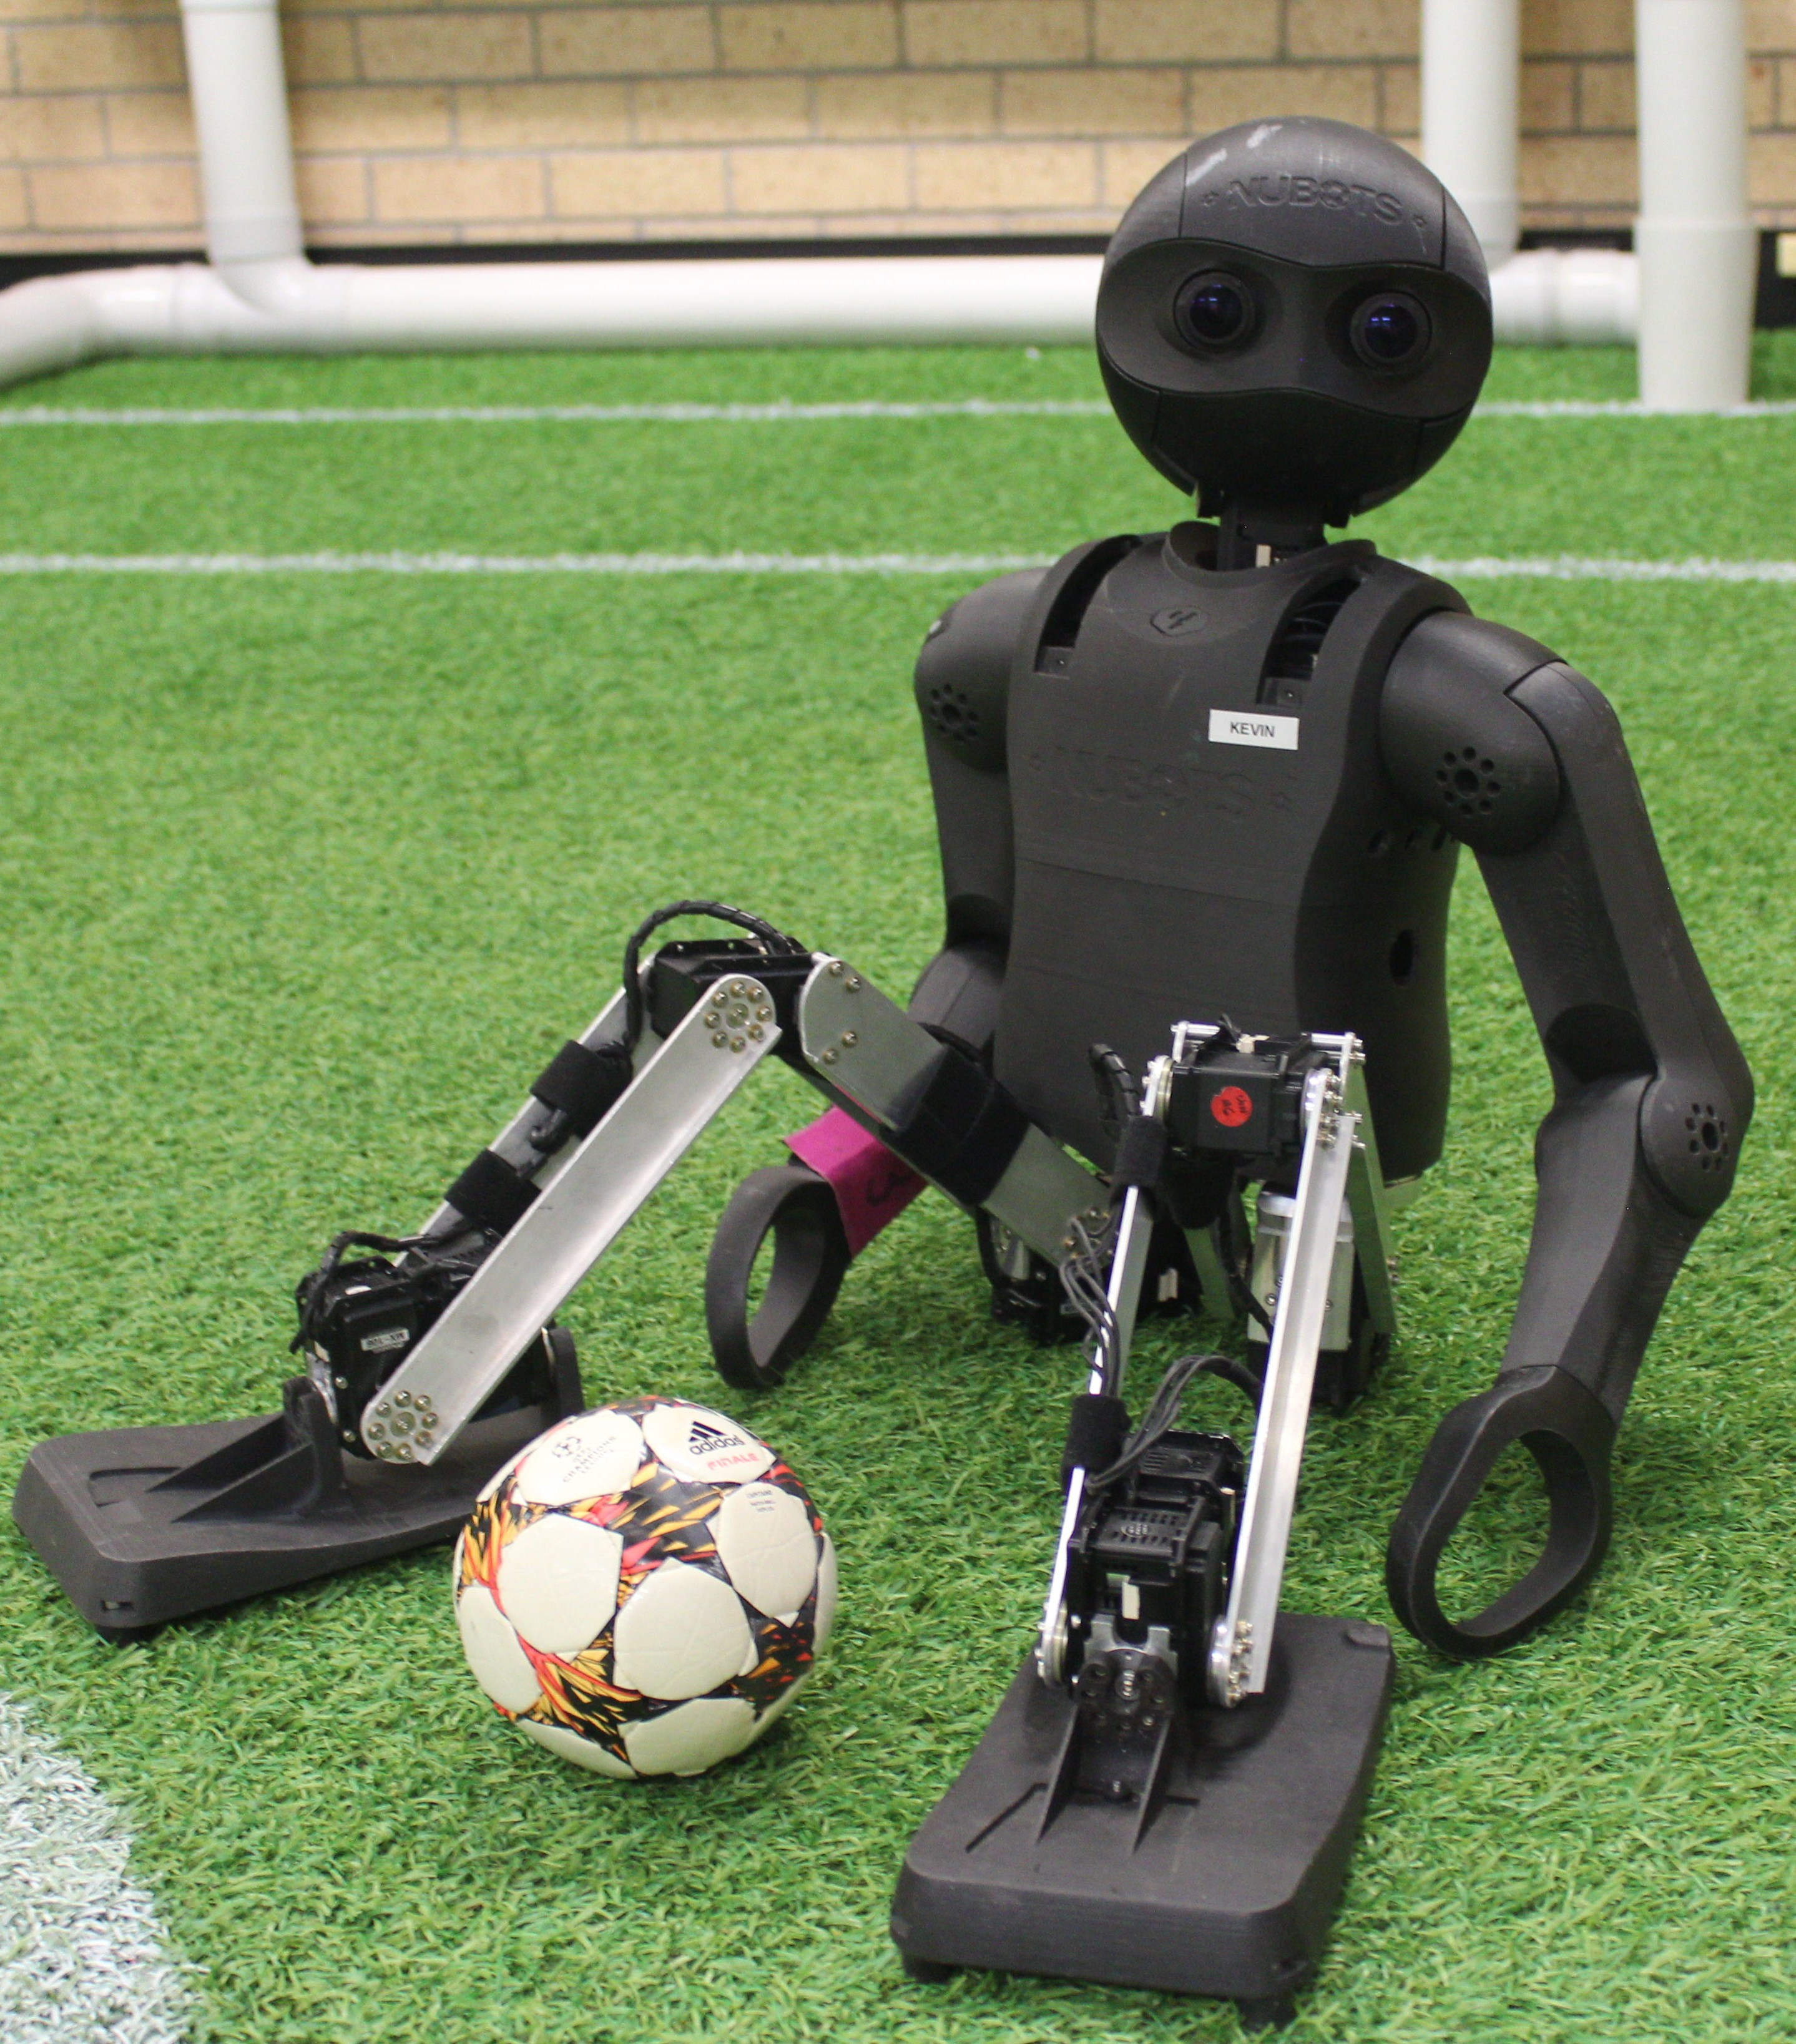
\includegraphics[width=0.47\textwidth]{Kev1}\\
		\textbf{NUgus Robot}.
	\end{center}
\end{figure}

\end{multicols}

\end{document}